\documentclass{article}
\usepackage[english]{babel}
\usepackage{amsthm}
\theoremstyle{definition}
\newtheorem{theorem}{Theorem}[section]
\newtheorem{corollary}{Corollary}[theorem]
\newtheorem{lemma}[theorem]{Lemma}
\usepackage[english]{babel}
\usepackage{amsmath,amsthm,amsfonts}
\usepackage{latexsym,amssymb}
\usepackage{graphicx}

\begin{document}
\section{Teorema}
\begin{theorem}
Sea $\psi$ una función de Orlicz tal que
\[\lim_{u \to \infty } \frac{\psi\left( u \right)}{u\log^{n-1}\left( u \right)} =0 \]\\
Entonces cada $f\in \psi(L)$ excepto las de un conjunto de primera categoría en $\psi(L)$ verifica que, para cada rotación $\gamma$ de $\mathbb{R}^n$,
\[\limsup_{R \in B_n}\frac{1}{\mu(R)}\int_{R}^{}\left| f\left( \gamma\left( y \right) \right) \right|d\mu\left( u \right)= +\infty  \]\\
para casi todo punto $x$.
\end{theorem}
\section {\normalsize EL PROBLEMA DE ANTONI ZYGMUND.}

Se trata del problema siguiente: sea $[0, \infty)×[0,\infty) \to [0,\infty), \phi (0,0) = 0$
, una función monótona creciente separadamente en cada variable. Por ejemplo, la función
\[\\phi\left( s,t \right)=s^\alpha t^\beta, \hspace{0.5cm} con \hspace{0.2cm}\alpha,\beta>0\]\\
Consideremos la colección biparamétrica $B_\phi$ de todos los paralelepípedos de $\mathbb{R}^3$, de lados paralelos a los ejes coordenados y cuyas dimensiones son de la forma: $s\times t \times \phi(s,t), s,t\in \mathbb{R}^+ $.\\
\begin{center}
    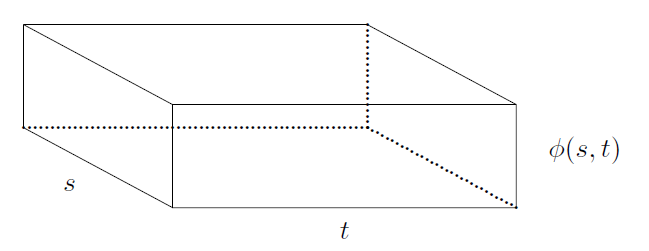
\includegraphics[scale=0.5]{pelosd.png}
\end{center}
\end{document}
